\documentclass[12pt,a4paper]{article}
\usepackage[utf8]{inputenc}
\usepackage[francais]{babel}
\usepackage[colorlinks=true,linkcolor=black,linktoc=all]{hyperref}
\usepackage[linesnumbered, ruled, french,onelanguage]{algorithm2e}
\usepackage{graphicx}
\usepackage[left=2cm,right=2cm,top=2cm,bottom=2cm]{geometry}
\usepackage{colortbl}
\usepackage[nottoc]{tocbibind}
\newcommand\tab[1][0.65cm]{\hspace*{#1}}
\SetKwRepeat{Do}{faire}{tant que}

\begin{document}
\begin{titlepage}
	\centering
	
\includegraphics[width=0.5\textwidth]{SU.jpg}\par\vspace{1cm}
	{\scshape\LARGE Sorbonne Université\\ Faculté des Sciences et Ingénierie \par}
	\vspace{1cm}
	{\scshape\large Master d'informatique \par}
	\vspace{1cm}
	{\scshape\Large 4I205 - Projet ANDROIDE\par}
	\vspace{1.5cm}
	{\huge\bfseries Rapport du projet :\\
		Nouvelle technique de visualisation en Interaction Homme-Machine\par}
	\vspace{2cm}
	{\Large\itshape B. Thanh Luong, 3504859 \\      Melissa Yaya, 3673113\par}
	\vspace{1cm}
	{Le projet est disponible sur : \href{https://github.com/leondoofus/IconHK}{https://github.com/leondoofus/IconHK}}
	\vfill
	Encadrant :\par
	M. Gilles Bailly
	\vfill

% Bottom of the page
	{\large mai 2018\par}
\end{titlepage}
\newpage
\tableofcontents
\newpage
\section{Résumé}
Dans le cadre de ce projet, nous implémentons des fonctionnalités d'une nouvelle perspective sur la conception des boutons de la barre d'outils qui vise
à augmenter l'accessibilité aux raccourcis clavier. \textbf{IconHK} met en œuvre cette perspective en mélangeant des repères visuels qui transmettent des informations de raccourci clavier dans les boutons de la barre d'outils sans dénaturer la représentation graphique de leur commande. Trois stratégies de conception ont été introduises pour intégrer le raccourci clavier et un encodage visuel
pour transmettre les modificateurs. Au cours de ce travail, nous développons un outil pour aider les concepteurs à appliquer le principe d'IconHK.
\section{Introduction}
Les boutons de la barre d'outils sont des widgets fréquemment utilisés pour la sélection des commandes. Ils sont conçus pour occuper une petit zone, mais ils transmettent beaucoup d'informations aux utilisateurs: l'icône est directement liée à la signification de la commande, la
couleur du bouton informe si la commande est disponible ou non, et la forme générale et l'effet d'ombre permet une interaction par "point \& click" pour exécuter la commande.\\
\tab Parce qu'ils sont concis et pratiques, les boutons de la barre d'outils sont devenus des widgets phares dans les interfaces graphiques (GUI). La plupart des commandes peuvent également être sélectionnées en utilisant un raccourci clavier associé.\\
\tab Les raccourcis clavier permettent aux utilisateurs d'atteindre des performances supérieures par rapport à la sélection d'une commande qui se fait en pointant et cliquant sur un bouton, en particulier pour les actions fréquentes telles que les opérations répétées de “Copier/Coller“.Les menus et les icônes de barres d'outils sont plus faciles à apprendre, tandis que les raccourcis clavier sont plus efficaces. Il semblerait naturel que les utilisateurs migrent de méthodes de menus et d'icônes simpliste, à une méthode plus efficace de raccourcis clavier au fur et à mesure qu’il gagne en expérience.\\
\tab Pour déterminer dans quelle mesure cette transition a lieu, 251 utilisateurs expérimentés de Microsoft Word ont reçu un questionnaire évaluant leur choix de méthodes pour les commandes les
plus fréquentes \cite{1} . Contrairement à nos attentes, la plupart des utilisateurs expérimentés utilisaient
rarement les raccourcis clavier, préférant l'utilisation des icônes de barre d’outils.
Plusieurs raisons peuvent expliquer ce comportement \cite{2}: Les utilisateurs pourraient ne pas être au courant de cette modalité, ils pourraient ne pas voir les gains d'efficacité, ou ils pourraient ne pas
être prêts à faire l'effort supplémentaire pour l'apprendre. Même lorsque les utilisateurs sont désireux d’apprendre un raccourci clavier, ils doivent actuellement naviguer dans un menu hiérarchique pour récupérer la combinaison de touches et la mémoriser explicitement pour une utilisation future. En d'autres termes, sélectionner une commande via son raccourci clavier n'est pas
aussi accessible qu'en pointant et en cliquant sur un bouton de la barre d’outils.\\
\tab Une deuxième étude a été faite pour vérifier que les raccourcis clavier sont, en effet, la méthode la plus efficace. Six participants ont exécuté des commandes communes en utilisant la sélection de
menu, les barres d'outils d'icônes et les raccourcis clavier. Les raccourcis clavier étaient, comme prévu, les plus efficaces \cite{1}. Ces études montrent que même les utilisateurs expérimentés sont inefficaces dans l'utilisation des interfaces graphiques.\\
\tab Un moyen possible d'améliorer l'efficacité de l'utilisateur consiste à ce que les programmes fournissent une cheat sheet, permettant aux utilisateurs de faire la transition entre l'utilisation des menus déroulants ainsi que le "point\& click" des icônes de la barre d’outils pour l'édition des raccourcis clavier. En effet, IconHK qui est le sujet de ce projet, prend place pour pallier ce problème, permettre la flexibilité de la technique d’interaction et un bon usage des raccourcis clavier.
\section{IconHK}
IconHK est une nouvelle technique d'interaction innovante qui a été proposée dans le domaine de l’Interaction Homme-Machine. Elle favorise l'utilisation des raccourcis clavier, plutôt que les
menus, pour sélectionner des commandes dans les GUIs et donc permet de gagner considérablement en efficacité.\\
\tab IconHK consiste à redesigner les icônes de la barre d'outils pour qu'elles communiquent non seulement la signification de la commande (e.g. une disquette pour la commande "Sauvegarder"), mais aussi le raccourci clavier (e.g Ctrl+S).\\
\tab Une telle approche allie des repères visuels transportant des raccourcis clavier dans les boutons de la barre d’outils pour permettre la reconnaissance visuelle du raccourci sans altérer la représentation
picturale de la commande existante. Elle vise également à relever des défis de conception que nous allons aborder plus bas.\\
\tab L’icône du bouton de la barre d’outils suggère la signification de la commande associée et son aspect permet de l'activer en cliquant dessus. Cependant, ce qu'un bouton de barre d'outils ne permet pas, c’est la méthode alternative pour exécuter la commande, à savoir le raccourci clavier - une combinaison de touches, typiquement une touche de modificateur (par exemple ctrl, alt) et une touche de raccourci (habituellement une lettre). Avec IconHK, nous visons à augmenter les boutons de la barre d'outils avec la capacité de suggérer cette façon de procéder à travers une meilleure exposition des raccourcis clavier. Cinq défis de conception liés à cet objectif ont été identifiés \cite{3}.
\subsection{Défis de conception d'IconHK}
\begin{enumerate}
\item {\large \textbf{Transmission des raccourcis clavier}}\\
Le premier défi consiste à transmettre efficacement les raccourcis clavier, c'est-à-dire à exposer explicitement leur existence aux utilisateurs. L'avantage est de permettre aux utilisateurs qui ne connaissent pas ou ne se rappellent pas des raccourcis, de les récupérer facilement.\\
\tab Deux approches principales ont été adoptées dans la plupart des applications pour communiquer les raccourcis clavier. L'une affiche les combinaisons de touches avec les éléments de menu. Dans ce cas, les utilisateurs ne sont exposés aux raccourcis qu'après avoir navigué dans la hiérarchie des
menus, ce qui nécessite un effort supplémentaire par rapport à un clic sur un bouton de la barre d'outils. L'autre fait en sorte de ressortir de la barre d'outils une info-bulle qui affiche le raccourci
après avoir survolé un bouton, moyennant un temps pour l’affichage de mais au prix d'attendre que l'info-bulle soit révélée si elle existe, sachant que les utilisateurs n'ont aucun moyen de le savoir et
répètent plusieurs fois cette action pour inspecter plusieurs raccourcis.\\
\tab Les deux approches ci-dessus s'appuient sur feedforward, qui consiste à présenter les informations aux utilisateurs avant d'exécuter la commande.\\
\tab D'autres travaux ont proposé une stratégie de feedback, où les informations sur le raccourci sont communiquées lors de l'exécution d'une commande, jouant le rôle d'une recommandation pour la prochaine fois. L'application Hotkey-Eve \cite{4} en est un exemple: chaque fois qu'un élément de menu
est sélectionné à l'aide de la souris, le raccourci clavier correspondant est indiqué dans le coin supérieur droit de l'écran. Hotkey Skillometer \cite{5} va un peu plus loin, et affiche des informations
concernant les combinaisons de touches, encourageant leur utilisation. Grossman et al. introduit une approche basée sur les coûts, qui désactive le menu afin de forcer les utilisateurs à utiliser les raccourcis. HotkeyCoach \cite{6} combine les approches de feedback et de coût: après chaque sélection de commande basée sur la souris, une fenêtre pop-up apparaît pour afficher la touche de raccourci correspondante. Les utilisateurs ne peuvent pas continuer tant qu'ils n'ont pas exécuté le raccourci
clavier ou fermé la fenêtre contextuelle.\\
\tab IconHK comprend des stratégies feedforward et feedback pour exposer les raccourcis clavier avec un minimum d'effort de la part des utilisateurs.
\item {\large \textbf{Maximisation de la durée d'exposition des raccourcis}}\\
Idéalement, l'aide visuelle pour rappeler les raccourcis devrait toujours être visible, mais dans la pratique, cette aide est généralement transitoire.\\
\tab Les méthodes transitoires affichent généralement l'aide visuelle à la demande, comme les info-bulles ou les aides de menu. Les approches qui fournissent une aide globale, hors contexte, nécessitent généralement que les utilisateurs effectuent des opérations explicites pour afficher/masquer des informations. C'est le cas avec ExposeHK \cite{7} et Cheat Sheet \cite{8}, où l'aide visuelle est affichée tant qu'une touche de modificateur est maintenue.\\
\tab Quelques méthodes permanentes qui affichent en permanence des mappages de raccourcis de commandes ont également été proposées. Par exemple, Hopper Disassembler \cite{9} utilise l'approche extrême consistant à afficher uniquement les raccourcis clavier sur les boutons de la barre d'outils, au détriment des icônes graphiques pour lesquelles il n'y a plus de place à afficher.\\
\tab Trop d'opérations pour accéder aux aides visuelles et/ou les masquer ralentissent l'interaction et interrompent le flux de travail. Cela peut produire une baisse de performance \cite{10} qui décourage
l'utilisation des raccourcis et piège les utilisateurs dans un "mode débutant" basé sur un pointeur \cite{12}.\\
\tab D'un autre côté, ces processus fastidieux peuvent parfois être perçus comme une incitation à motiver les utilisateurs à apprendre des raccourcis \cite{6}.\\
\tab IconHK vise à maximiser la durée d’exposition, établissant un équilibre entre une bonne communication des raccourcis, une minimisation d’efforts et cela sans perturber l’utilisateur. À cette fin, il prend en charge à la fois l'exposition transitoire et permanente, offrant différents
compromis entre la lisibilité et la durée de l’exposition.
\item {\large \textbf{Minimisation de l'espace visuel pour la transmission de raccourcis}}\\
L'affichage des combinaisons de touches nécessite un espace visuel, ce qui n'est pas toujours possible ni souhaitable. La dimension limité des écrans est la principale raison pour laquelle les techniques ci-dessus ont été développées.\\
\tab Plusieurs approches constituent explicitement de l'espace pour s'adapter aux raccourcis. Par exemple, les menus sont élargis pour ajouter des aides visuelles aux éléments de menu, mais des combinaisons plus complexes ont tendance à donner lieu à des menus trop volumineux.\\
\tab Une autre approche consiste à masquer temporairement une partie de l'interface graphique pour afficher le raccourci, comme le font les info-bulles ou ExposeHK. Le cas d'ExposeHK \cite{7} est intéressant, car il définit avec succès un mécanisme pour afficher des informations pertinentes, mais
ne parvient pas à afficher les informations sans masquer une partie de l'interface graphique.\\
\tab IconHK améliore et complète les travaux antérieurs en proposant différentes stratégies pour mélanger les raccourcis clavier dans le pictogramme.\\
\tab Plusieurs approches dans la littérature proposent de mélanger des informations avec des éléments visuels déjà en place sans les obscurcir. Des icônes animées ont été conçues pour transmettre plus
explicitement la signification d'une commande en prévisualisant son résultat \cite{11}. FatFont \cite{12}, bien
que moins apparenté, est un exemple intelligent de police optimisée pour l'espace(chiffres seulement), où la quantité de pixels sombres dans un caractère numérique est proportionnelle au nombre qu'il représente et où les nombres multi-chiffres sont imbriqués. que chaque nombre occupe
le même espace visuel qu'un seul chiffre.\\
\tab IconHK s'appuie sur cette dernière catégorie d'approches consistant à mélanger de nouvelles informations sans perturber la mise en page.
\item {\large \textbf{Transmettre la signification des commandes}}\\
IconHK partage l'objectif principal des icônes informatiques existantes: communiquer la signification des commandes. À cette fin, une icône doit être sémantiquement liée à la signification de la commande, être compréhensible et se distinguer des autres icônes.\\
\tab L'impact des caractéristiques des icônes sur la recherche visuelle a été étudié [13,14]. Ces caractéristiques comprennent la concordance, la complexité, la taille et la forme qui sont liées à la
compréhensibilité et à la distinction. En particulier, la complexité visuelle des icônes augmente le temps de recherche même après de nombreux essais, car "cela nécessite un temps de traitement
supplémentaire pour lier toutes les fonctionnalités de l'icône afin d’en comprendre la fonction" \cite{14,15}.\\
\tab IconHK vise à intégrer à la fois les informations sur le raccourci clavier et la représentation graphique de la commande dans le même bouton de la barre d'outils. Le principal défi avec cet objectif est de garantir que les icônes de la barre d'outils restent compréhensibles et identifiables.
\item {\large \textbf{Le maintient de l'attrait esthétique des icônes}}\\
En plus de communiquer la signification des commandes impliquées dans un logiciel, les icônes de la barre d'outils contribuent à l'esthétique globale de l'interface, qui est un facteur critique de l'expérience de l'utilisateur \cite{16}. L'attrait esthétique est lié à de nombreux critères et dépend de la perception personnelle des utilisateurs. La familiarité et la complexité de l'icône peuvent facilement
influencer l'attrait esthétique de l'icône \cite{17}. Alors que les décisions esthétiques liées à l'aspect visuel de la représentation graphique de la commande sont laissées au concepteur, IconHK se propose d'être aussi peu destructrice que possible afin de conserver un attrait esthétique aussi élevé que les visuels originaux.
\end{enumerate}
\subsection{Incorporation de raccourcis clavier dans les boutons de la barre d’outils}
Notre objectif initial consiste à intégrer des repères visuels transportant le raccourci clavier et les modificateurs dans un bouton, ce qui implique d'intégrer le symbole et les indicateurs sur les
modificateurs tout en préservant l'esthétique et la lisibilité du pictogramme.
Inspiré par les design de logo \cite{18}, trois stratégies ont été proposées pour intégrer un symbole dans l'icône d'un bouton \cite{3} :
\begin{enumerate}
\item {\large \textbf{L’espace vide}}\\
Consiste à tirer parti de l'espace vide dans ou autour du pictogramme pour afficher le symbole. Par exemple, seulement 23\% des pixels de l’icône 
\includegraphics[width=0.04\textwidth]{i1.png} sont consacrés au pictogramme, ce qui laisse suffisamment de place en haut à gauche du bouton pour intégrer la lettre 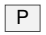
\includegraphics[width=0.04\textwidth]{i2.png}. L'icône 
\includegraphics[width=0.04\textwidth]{i3.png} a un grand
espace vide dans son pictogramme qui est suffisant pour insérer le symbole 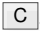
\includegraphics[width=0.04\textwidth]{i4.png}. La stratégie est limitée aux icônes avec peu de pixels peints ou contenant de grandes zones uniformes. Plusieurs icônes telles que 
\includegraphics[width=0.04\textwidth]{i5.png} ou 
\includegraphics[width=0.04\textwidth]{i6.png} n’offrent pas suffisamment d'espace pour incorporer un symbole tel quel.
(figure 1)
\begin{center}
	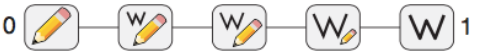
\includegraphics[width=0.5\textwidth]{T1.png}\\
	Figure 1: stratégie de l’espace vide
\end{center}
\item {\large \textbf{L’espace positif}}\\
Consiste à révéler le symbole de la silhouette du pictogramme. Cette stratégie est souvent utilisée par les concepteurs de logo pour mélanger de manière transparente du texte et des images dans un seul visuel ou utiliser des objets de formes particulières pour évoquer des lettres \cite{18}. Cette stratégie est mieux illustrée par l'icône 
\includegraphics[width=0.04\textwidth]{i7.png} en forme de ciseaux de la commande 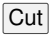
\includegraphics[width=0.04\textwidth]{i8.png} dont la forme du
pictogramme ressemble à la lettre 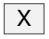
\includegraphics[width=0.04\textwidth]{i9.png} du raccourci correspondant. Peut-être pour des raisons esthétiques, différentes orientations des ciseaux sont courantes, par ex. 
\includegraphics[width=0.04\textwidth]{i10.png}, ce qui rend la perception
du raccourci plus difficile. Idéalement, le symbole dérivé de la forme générale ou des  bords du pictogramme doit être aussi droit que possible pour s'assurer que l'icône communique le mieux la signification et le raccourci clavier. L'icône 
\includegraphics[width=0.04\textwidth]{i11.png} est un autre exemple où le raccourci 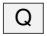
\includegraphics[width=0.04\textwidth]{i12.png} ou 
\includegraphics[width=0.04\textwidth]{i3.png} peut facilement être dérivé mais, comme avec l'espace vide, toutes les icônes ne sont pas qualifiées pour cette approche. Certains pictogrammes ne supportent pas facilement un symbole codé par l'accentuation des bords, tels que 
\includegraphics[width=0.04\textwidth]{i14.png}. (figure 2)
\begin{center}
	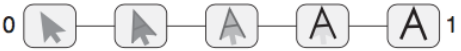
\includegraphics[width=0.5\textwidth]{T2.png}\\
	Figure 2: stratégie de l’espace positif
\end{center}
\item {\large \textbf{L’espace négatif}}\\
Consiste à exploiter l'espace libre autour d'un objet pour déguiser une lettre. Cet effet visuel, populaire dans la création de logo \cite{18}, s’appuie sur une ambiguïté de la figure qui crée un visuel offrant deux points de vue alternatifs, une technique d'illusion commune qui découle des principes
de Gestalt \cite{19}. Un exemple bien connu est le vase de Rubin \cite{20} où l'espace positif blanc forme un vase, tandis que l'espace négatif noir forme deux visages sur le point de s’embrassé. Les lettres fermées telles que 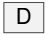
\includegraphics[width=0.04\textwidth]{i15.png} ou 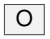
\includegraphics[width=0.04\textwidth]{i16.png} peuvent être facilement dissimulées dans l'espace négatif d'une icône dont le pictogramme ressemble à une forme ronde. En revanche, l'illusion devient plus difficile à obtenir avec des lettres ouvertes (par exemple 'J', 'E'), car les pictogrammes ne sont généralement pas confondus avec les bordures des icônes (l'espace négatif ne peut donc pas donner une lettre ouverte). Un autre mécanisme cognitif peut aider dans ces cas: le principe Gestalt de la fermeture,
qui fait référence à la tendance de notre esprit à percevoir des formes complètes même si une image est incomplète. Ce mécanisme est bien illustré par la lettre 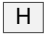
\includegraphics[width=0.04\textwidth]{i17.png} que l'icône 
\includegraphics[width=0.04\textwidth]{i18.png} peut évoquer. Bien qu'il ne corresponde pas exactement à l'espace négatif du pictogramme, 'H' peut être déduit de la forme du pictogramme global par la fermeture. (figure 3)
\begin{center}
	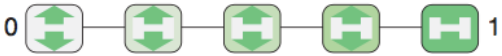
\includegraphics[width=0.5\textwidth]{T3.png}\\
	Figure 3: stratégie de l’espace négatif
\end{center}
\end{enumerate}
\tab Deux études ont été menées \cite{8}, la première examine les avantages d'IconHK pour les utilisateurs finaux en évaluant l'efficacité de la récupération des raccourcis clavier des différentes stratégies. Les résultats suggèrent que les stratégies spatiales positives et négatives sont des aides mnémoniques utiles.\\
\tab Une deuxième étude fournit des idées de concepteurs professionnels sur la praticité de l'approche IconHK. Les résultats indiquent que la stratégie de l'espace vide est préférée pour sa simplicité et sa
pertinence pour les styles minimalistes, et pointent vers des défis de conception, en particulier pour maintenir la cohérence de l'ensemble d'icônes, pour les deux autres stratégies.\\
\tab Dans ce projet nous nous intéresserons à une seule stratégie qui est préférée dans la deuxième étude,
celle de l’espace vide.
\subsection{Modificateurs d’intégration}
L'incorporation du symbole de raccourci unique dans une icône est suffisante lorsque les raccourcis clavier n'impliquent pas de touches de modification ou lorsque les raccourcis impliquent systématiquement le même modificateur, généralement Ctrl. Lorsque différents modificateurs sont
impliqués dans la même application, d'autres indications sont nécessaires.\\
\tab L'incorporation d'une représentation graphique ou textuelle de touches de modification peut considérablement augmenter la complexité de l'icône et affecter sa lisibilité.\\
\tab Pour générer des codages visuels possibles des modificateurs, des idées ont été suscitées de la part de quatre experts HCI non impliqués dans la conception d’IconHK \cite{3}. Une idée fréquemment
proposée consiste à associer chaque touche modificatrice à un carré situé à l'un des quatre coins du bouton, où un carré est rempli lorsque le modificateur correspondant est utilisé par le raccourci et
vide autrement \cite{3}, tel qu'illustré à la figure 4.\\
\tab Pour une cohérence visuelle du design, un des expert a proposé: "chaque touche de modification peut être mappée de manière stable sur un coin du bouton, en fonction de sa position physique sur le clavier: Alt en bas à droite, Ctrl en bas à gauche et Shift en haut à gauche".\\
\tab Différents indicateurs visuels peuvent être envisagés, mais dans le but de minimiser l’espace visuel
occupé, un quart de cercle a été utilisé au lieu de carrés \cite{3}. Cette conception offre également un
codage d'état plus riche: lorsqu'un utilisateur appuie sur une touche de modification spécifique, le
coin correspondant est mis en surbrillance sur tous les boutons de la barre d’outils afin d'aider les
utilisateurs à découvrir ce mappage (par exemple, le coin inférieur gauche est surligné en bleu lors
de la commande Ctrl sur la figure 4, à droite).
\begin{center}
	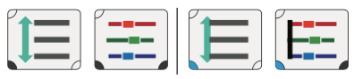
\includegraphics[width=0.5\textwidth]{T4.png}\\
	Figure 4: Exemple d'icônes augmentées avec IconHK qui incorpore des modificateurs à l'aide de la
	fonction d'insertion de clé par clavier.
\end{center}
\section{Travail à réaliser}
Notre groupe est constitué de deux étudiants. Pour mener à bien notre projet, nous avons proposé un planning prévisionnel des tâches à accomplir par chaque membre de l’équipe.\\
\tab Avant tout, nous avons commencé par nous documenter, ce qui nous a permis de cerner le sujet comme il se doit. Puis chaque membre a étudié une partie plus en détail (création des boutons de la barre d’outils, l’activation de l’animation, etc.), qu’il s’est chargé d’expliquer au second membre durant nos séances de travail.\\
\tab En outre, le projet a été divisé en deux parties distinctes, la première partie étant dédiée à la programmation dont la complétion d'un démonstrateur d'IconHK et au développement de la stratégie de l'espace vide ainsi que l'intégration notre API dans des applications open source, et la seconde, à la recherche bibliographique et la rédaction de ce rapport. Nous assistions à une réunion toutes les semaines avec notre encadrant. Cette réunion a pour but de faire le point sur l’état d’avancement du projet et d’éclaircir d’éventuelles ambiguïtés.\\
\subsection{Dévéloppement de l'API}
Partant de l'héritage de la classe \texttt{JButton}, le projet a pour but de redessiner le composant graphique et de ne pas changer la fonction principale du bouton. La surcharge des méthodes graphiques ne complexifie pas l'ensemble de l'application car ces méthodes sont appelées automatiquement quand nous utilisons l'interface graphique (i.e boucle infinie). Une deuxième alternative est d'encapsuler le bouton dans une classe puis nous pouvons changer ses propriétés avec des méthodes personnalisées. Cette deuxième solution est réalisable mais elle n'est pas pratique. Nous voulons que notre API soit le plus simple possible, c'est-à-dire l'utilisateur n'a qu'à changer quelques lignes de code en passant de \texttt{JButton} à \texttt{HKButton} et cela ne détruira pas toute la structure du code.
\begin{enumerate}
\item {\large \textbf{L'espace vide}}\\
Dans un premier temps, nous fournissons un répertoire contenant toutes les lettres représentant les raccourcis (\texttt{IconHK/resources/icons}) qui nous permet de générer une séquence d'images pour l'animation d'un bouton. Nous proposons 3 types de génération de la séquence : linéaire, quadratique et cubique. L'espace occupé d'un bouton est divisé en 2 parties : une pour l'icône principal et l'autre pour la lettre représentant le raccourci. Le ratio de la lettre par rapport à la zone entière varie en fonction du temps (dans notre cas c'est la position du cadre courant). Nous générons une séquence de 25 images pour chaque bouton. À l'état initial (0) le bouton est complètement peint avec l'icône principal et contrairement, à l'état final (25) il contient uniquement la lettre. À n'importe quel état intermédiaire entre ces deux, il est peint avec un ratio calculé en fonction de l'état et du style choisi.
\begin{center}
	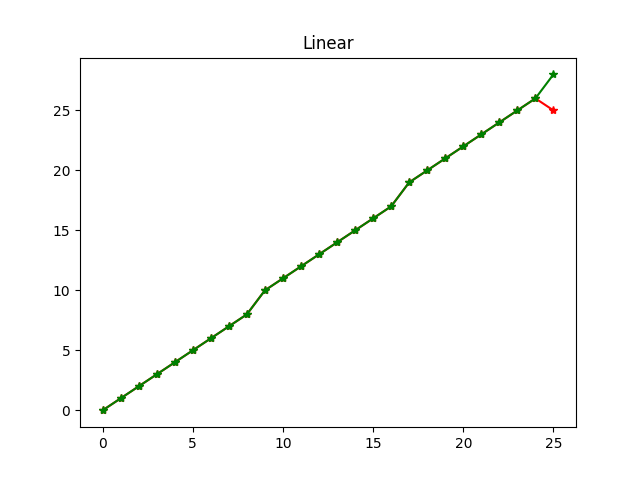
\includegraphics[width=0.4\textwidth]{linear.png}
	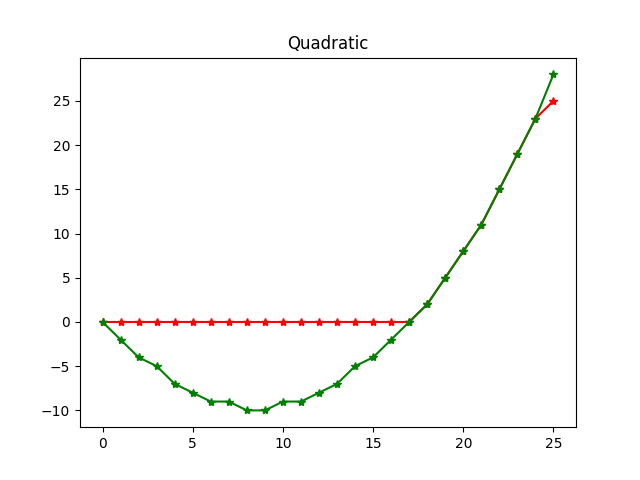
\includegraphics[width=0.4\textwidth]{quadratic.png}
	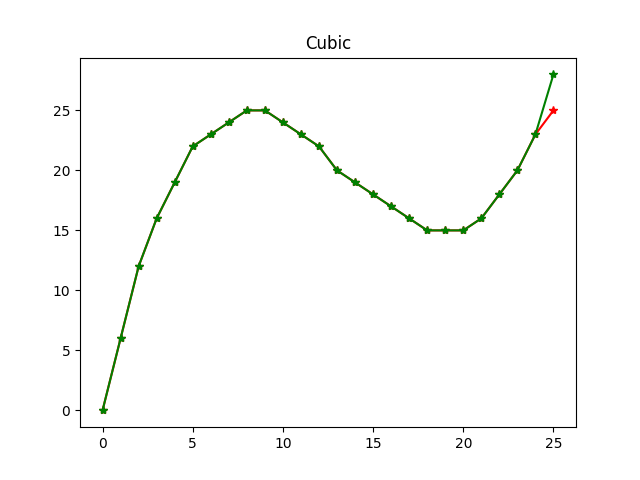
\includegraphics[width=0.4\textwidth]{cubic.png}
\end{center}
Pour une taille de 50 pixels, le ratio est calculé sachant les point supplémentaires puis fixé pour que l'image soit rentable.
Les courbes ne sont pas lisses parce que l'arrondi et le convertissement des nombres réels en nombres entiers ne le permettent pas. Les courbes vertes obtenues par calcul et les rouges sont fixées pour que l'image soit visible dans le bouton. Par exemple, avec la fonction linéaire, au cinquième cadre la lettre occupe $\frac{5}{25}$ soit 20\% l'espace du bouton et 80 \% pour l'icône, etc.. Les courbes des fonctions quadratique et cubique sont obtenues grâce à la méthode de Cramer. Nous introduisons des points intermédiaires afin de calculer ces courbes. Pour la fonction quadratique nous mettons p=(20,0.3) comme point de contrôle et p$_1$=(8,0.9), p$_2$=(14,0.7) pour la cubique.
Nous avons pensé à introduire des fonctions plus complexes (comme la Courbe de Bézier) mais elles complexifieront le comportement des utilisateurs.\\
Nous pouvons constater que la fonction quadratique est assez inutile car pendant 17 premier cadres, il n'y aucune animation. Cependant, la fonction cubique crée un effet rebond très intéressant.
\item {\large \textbf{Aspect IHM}}\\
\begin{enumerate}
\item {\large \textbf{Raccourci}}\\
Nous proposons 2 types de visualisation l'animation :
\begin{itemize}
\item \textbf{Lock Hotkey} : Quand l'utilisateur appuie sur le modificateur associé au bouton, le bouton augment le cadre qui est sur la zone de dessin chaque 25m/s jusqu'à ce que le modificateur soit relâché ou l'état final soit atteint. Puis il revient au fur et à mesure à l'état initial quand l'utilisateur relâche le modificateur.
\item \textbf{Unlock Hotkey} : L'animation est activée jusqu'à ce que l'utilisateur relâche le modificateur. L'image affiché change de l'état initial à l'état final puis revient au initial, etc.
\end{itemize}
\item {\large \textbf{Clic}}\\
Un clic est généralement rapide, donc l'animation va aller jusqu'à l'état final puis revenir à l'état initial. Si la souris est maintenue sur le bouton, l'animation marche comme le cas Lock Hotkey.
\item {\large \textbf{MenuItem}}\\
Si l'action associée au bouton est encapsulée par \texttt{HKAction} fournie dans notre API, quand on clique sur un MenuItem, l'animation du bouton reliée à l'action est activée pour rappeler l'utilisateur du raccourci.
\end{enumerate}
\item {\large \textbf{"Apprentissage"}}\\
Nous rassemblons toutes les accessibilités d'une fonctionnalité dans notre \texttt{HKAction} qui à la fois lance la fonctionnalité et fait l'animation. Nous testons à chaque fois si la fonctionnalité est activée par un raccourci, un clic ou un MenuItem. Si c'est un clic ou un MenuItem, l'état initial du bouton est incrémenté de 1 pour faire apparaître la lettre au fur et à mesure. Il est décrémenté de 1 si c'est un raccourci. 
\item {\large \textbf{Paramétrage de l'icône}}\\
\begin{center}
	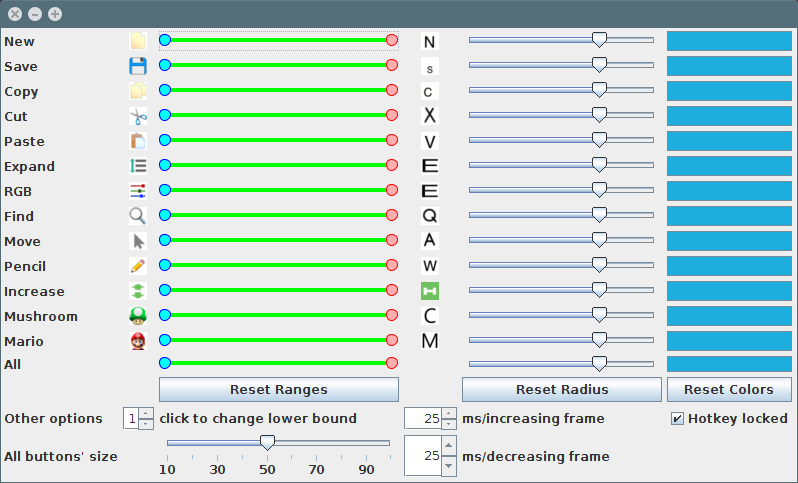
\includegraphics[width=0.8\textwidth]{11.png}
\end{center}
Nous proposons quelques paramètres pour que l'utilisateur puisse "jouer" avec notre projet. Nous pouvons paramétrer l'état initial, l'état final, la taille et la couleur du modificateur. La ligne "All" permet de paramétrer l'ensemble de tous les HKButtons utilisés. Dans ce panneau de configuration, nous pouvons définir le nombre de clics présenté dans la section "Apprentissage" et la vitesse de transition ainsi que la taille des boutons.
\end{enumerate}
\subsection{Intégration dans des applications open source}
Partant d'un démonstrateur, nous espérons d'intégrer notre API dans des applications open source. Nous avons choisi une première application simple qui ressemble à notre démonstrateur mais avec des fonctionnalités implémentées. Une deuxième application est beaucoup plus complexe mais elle est dans le marché depuis 11 ans. Les lignes en commentaire sont le code source et celles en rouges sont ajoutées pour utiliser notre API.
\begin{enumerate}
\item {\large \textbf{\href{https://github.com/pH-7/Simple-Java-Text-Editor}{Simple Java Text Editor}}}\\
\begin{center}
	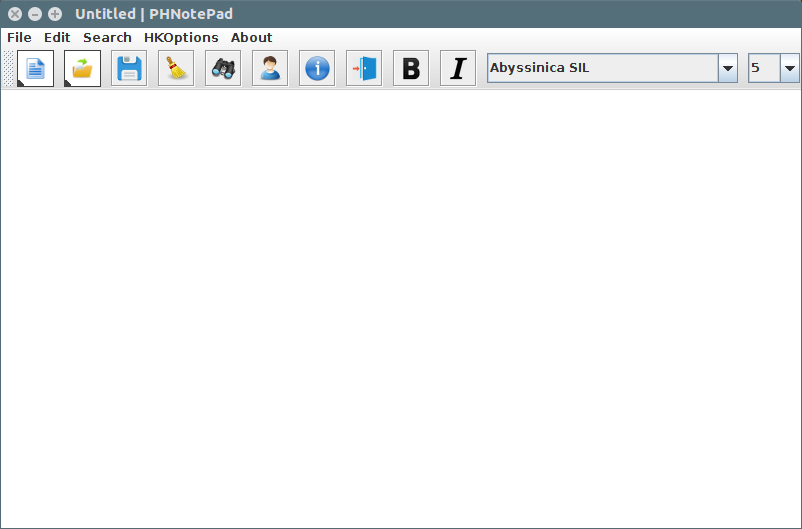
\includegraphics[width=0.8\textwidth]{01.png}\\
	La première application ressemble apparemment à notre démonstrateur.
\end{center}
En changeant quelques lignes de code, nous avons pu intégrer notre API dans cette application.
\begin{center}
	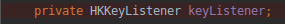
\includegraphics[width=0.4\textwidth]{02.png}\\
	Rajout notre Listener\\
	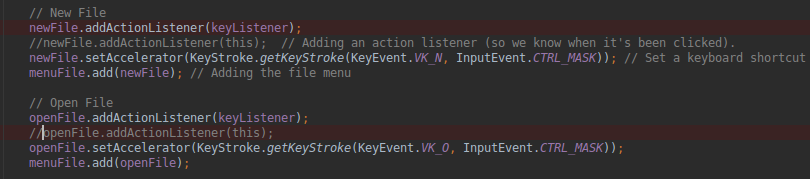
\includegraphics[width=0.9\textwidth]{04.png}\\
	Change leur listener au notre\\
	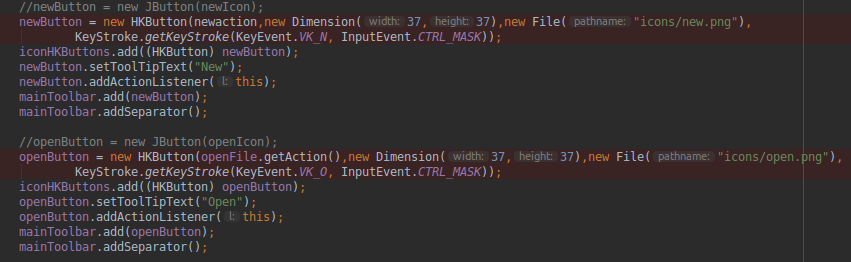
\includegraphics[width=0.9\textwidth]{06.png}\\
	Crée les boutons suivant notre prototype\\
	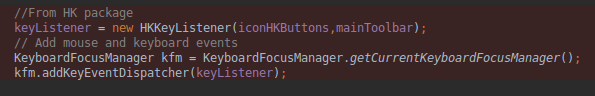
\includegraphics[width=0.9\textwidth]{07.png}\\
	Passe tous les HKButtons au listener
\end{center}
Jusqu'ici la création des boutons est faite. Nous constatons que quelques changements peuvent transformer un \texttt{JButton} simple à un \texttt{HKButton} animé.\\
Nous pouvons rajouter un MenuItem pour paramétrer les propriétés (ce qui est facultatif):
\begin{center}
	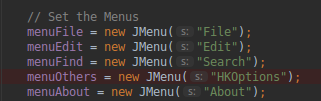
\includegraphics[width=0.5\textwidth]{03.png}\\
	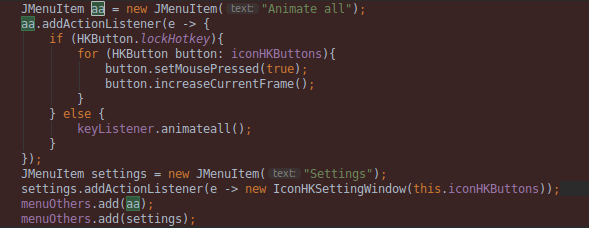
\includegraphics[width=0.9\textwidth]{05.png}\\
	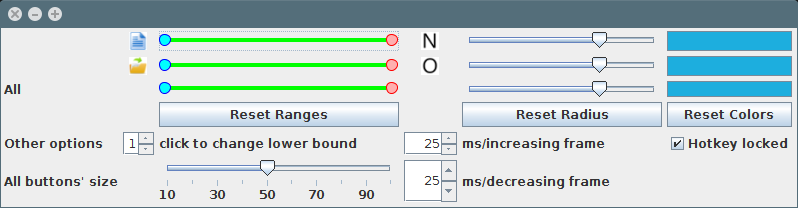
\includegraphics[width=0.9\textwidth]{16.png}\\
\end{center}
\item {\large \textbf{\href{https://github.com/Vanuan/sweethome3d}{Sweet Home 3D}}}\\
\textit{Package requis : java3d}\\
Même si cette application est plus complexe mais l'utilisation d'IconHK reste très simple :
\begin{center}
	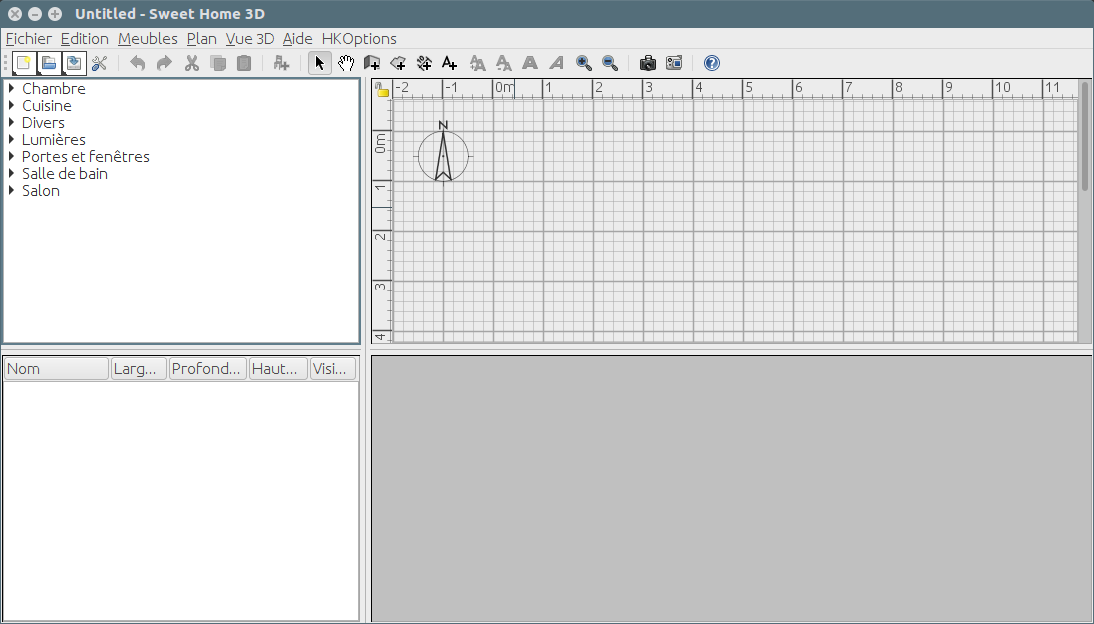
\includegraphics[width=0.9\textwidth]{08.png}\\
	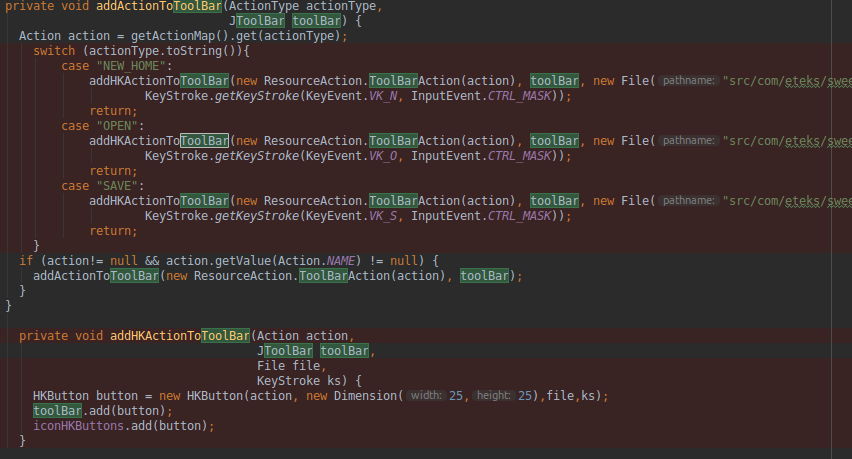
\includegraphics[width=0.9\textwidth]{10.png}\\
	Création des boutons\\
\end{center}
Le fait que \texttt{HKAction} encapsule seulement une \texttt{Action} simple qui est une limite de notre API.
Dans cette application, les actions associées au MenuItem sont très complexes. L'auteur a utilisé une \texttt{ActionMap} qui n'est pas compatible avec notre \texttt{HKAction} donc nous n'avons pas réussi à intégrer un aspect de notre modèle d'IHM.\\
L'ajout du panneau de configuration est comme dans l'application précédente :
\begin{center}
	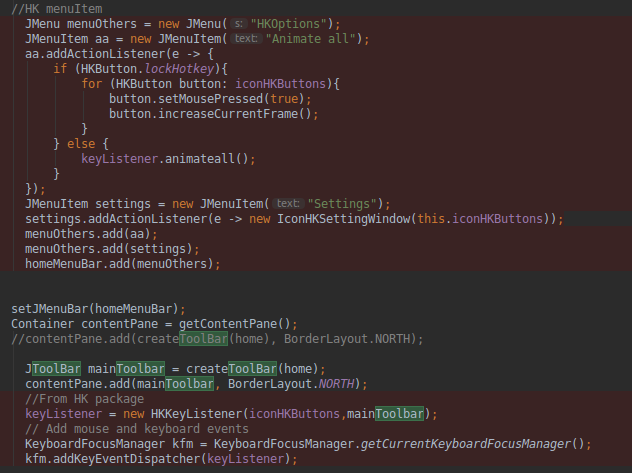
\includegraphics[width=0.9\textwidth]{09.png}\\
	Ajout le panneau de configuration\\
	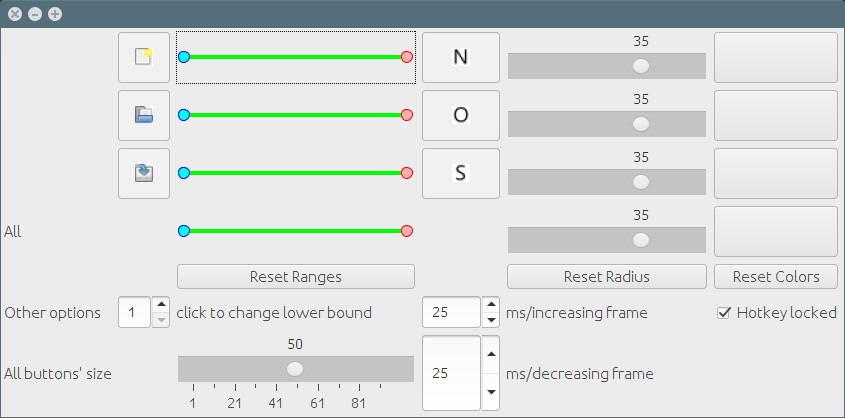
\includegraphics[width=0.4\textwidth]{13.png}
	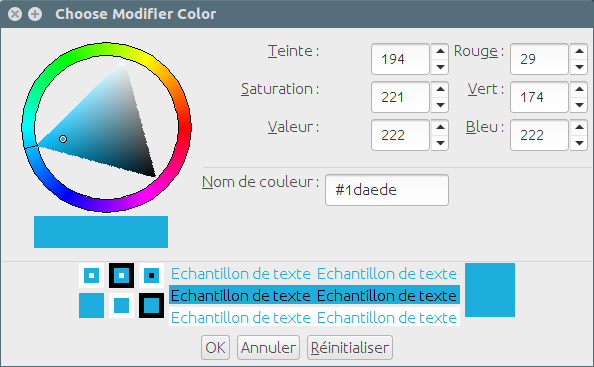
\includegraphics[width=0.4\textwidth]{14.png}\\
	Le créateur de l'application préfère le style de MacOS
\end{center}
\end{enumerate}
\section{Conclusion}
Bien que les interfaces utilisateur graphiques fournissent plusieurs méthodes de sélection des commandes, elles maintiennent généralement de nombreux utilisateurs dans un optimum local de performance où ils continuent à pointer et cliquer sur les boutons de la barre d'outils au lieu de
passer aux raccourcis clavier. Une raison pourrait être que les concepteurs d'interface ne traitent pas le problème de la sélection de commande dans son ensemble, c'est-à-dire que le choix du nom de la commande, de l'icône et du raccourci clavier n'est pas entièrement pris en compte.\\
\tab Avec IconHK, nous visons à renforcer la relation entre ces composants: l'icône doit communiquer à la fois la signification de la commande et son raccourci clavier. Cependant, concevoir des icônes est un exercice complexe impliquant des objectifs multiples (parfois contradictoires). Les concepteurs doivent équilibrer plusieurs objectifs tels que l'efficacité, la cohérence ou l'esthétique. Mais jusqu'à
présent, communiquer le raccourci clavier a été considéré comme un objectif majeur.\\
\tab Nous espérons que cette nouvelle perspective sur la conception d'icônes, et notre exploration du concept IconHK, catalyseront de nouveaux efforts visant à adopter une approche plus holistique de la conception graphique.\\
\tab Comme IconHK adresse un défi difficile de la conception d'icônes, plusieurs questions restent ouvertes pour le travail futur. En particulier, les recherches futures devraient déterminer si IconHK est approprié pour la plupart des applications dans le marché, tirer des méthodes pour aider les novices à comprendre le principe IconHK.
\newpage
\begin{thebibliography}{20}
\bibitem{1} Lane, D., Napier, A., Peres, C., and Sandor, A.. «The Hidden Costs of Graphical User Interfaces : The Failure to Make the Transition from Menus and Icon Tool Bars to Keyboard Shortcuts», \textit{International Journal of Human-Computer Interaction}. vol. 18, no 2, p. 133-144,
mai 2005.
\bibitem{2} Cockburn, A., Gutwin, C., Scarr, J., and Malacria, S.. «Supporting Novice to Expert Transitions in User Interfaces», \textit{ACM Comput. Surv.}. vol. 47, no 2, p. 31:1–31:36, nov. 2014.
\bibitem{3} Giannisakis, E., Bailly, G., Malacria, S., Chevalier F.. «IconHK : Using Toolbar Button Icons to Communicate Keyboard Shortcuts». in \textit{Proceedings of the 2017 CHI Conference on Human Factors in Computing Systems}, New York, NY, USA, 2017. p. 4715–4726.
\bibitem{4} Hotkey-eve: \href{http://www.hotkey-eve.com}{http://www.hotkey-eve.com}.
\bibitem{5} Malacria, S., Scarr, J., Cockburn, A., Gutwin, C., and Grossman, T.. «Skillometers: Reflective Widgets That Motivate and Help Users to Improve Performance», in \textit{Proceedings of the 26th Annual ACM Symposium on User Interface Software and Technology}, New York, NY, USA, 2013. p. 321–330.
\bibitem{6} Krisler, B., and Alterman, R.. «Training Towards Mastery: Overcoming the Active User Paradox», in \textit{Proceedings of the 5th Nordic Conference on Human-computer Interaction: Building Bridges}, Building Bridges, New York, NY, USA, 2008. p. 239–248.
\bibitem{7} Malacria, S., Bailly, G., Harrison, J., Cockburn, A., and Gutwin, C.. «Promoting Hotkey Use Through Rehearsal with ExposeHK», in \textit{Proceedings of the SIGCHI Conference on Human Factors in Computing Systems}, New York, NY, USA, 2013. p. 573–582.
\bibitem{8} Cheat sheet: \href{http://www.mediaatelier.com/cheatsheet/}{http://www.mediaatelier.com/cheatsheet/}.
\bibitem{9} Hopper disassembler «Eve Get Started»,: \href{http://hopperapp.com}{http://hopperapp.com}.
\bibitem{10} Scarr, J., Cockburn, A., Gutwin, C., and Quinn, P.. «Dips and Ceilings: Understanding and
Supporting Transitions to Expertise in User Interfaces», in \textit{Proceedings of the SIGCHI Conference on Human Factors in Computing Systems}, New York, NY, USA, 2011. p. 2741–2750.
\bibitem{11} Baecker, R., Small, I., and Mander, R.. «Bringing icons to life», in \textit{Proceedings of the SIGCHI Conference on Human Factors in Computing Systems}, New York, NY, USA, 1991, 1–6.
\bibitem{12} Nacenta, M., Hinrichs, U., and Carpendale, S.. «Fatfonts: Combining the symbolic and visual aspects of numbers», in \textit{Proceedings of the International Working Conference on Advanced Visual Interfaces}, New York, NY, USA, 2012. p. 407–414.
\bibitem{13} Gittins, D.. «Icon-based human-computer interaction», \textit{International Journal of Man-Machine Studies}. vol. 24, no 6, p. 519-543, juin 1986.
\bibitem{14} McDougall, S., Tyrer, V., and Folkard, S.. «Searching for signs, symbols, and icons: Effects of time of day, visual complexity, and grouping», \textit{Journal of Experimental Psychology: Applied}. vol. 12, no 2, p. 118-128, 2006.
\bibitem{15} McDougall, S. J., de Bruijn, O., and Curry, M. B.. «Exploring the effects of icon characteristics on user performance: The role of icon concreteness, complexity, and distinctiveness», \textit{Journal of Experimental Psychology: Applied}. vol. 6, no 4, p. 291306, 2000.
\bibitem{16} Ma, X., Matta, N., Cahier, J.-P., Qin, C., and Cheng, Y.. «From action icon to knowledge icon: Objective-oriented icon taxonomy in computer science», \textit{Displays}. vol. 39, p. 6879, oct.
2015.
\bibitem{17} McDougall, S. J., and Reppa, I.. «Why do i like it? The relationships between icon characteristics, user performance and aesthetic appeal», in \textit{Proceedings of the Human Factors and Ergonomics Society Annual Meeting}. vol. 52, no 18, p. 1257-1261, sept. 2008.
\bibitem{18} Silver, L.. «Graphic Design that Works: Secrets for Successful Logo, Magazine, Brochure, Promotion and Identity Design. Rockport», 2004.
\bibitem{19} Tuck, M.. «Gestalt principles applied in design». August 2010.
\bibitem{20} Rubin, E.. «Synsoplevede figurer». 1915.
\end{thebibliography}
\end{document}